\iffalse
\documentclass[journal,12pt,twocolumn]{IEEEtran}
\usepackage{amsmath,amssymb,amsfonts,amsthm}
\usepackage{txfonts}
\usepackage{tkz-euclide}
\usepackage[margin=0.25in]{geometry}
\usepackage{pgfplots}
\usepackage{listings}
\usepackage{gvv}
\usepackage[latin1]{inputenc}
\usepackage{adjustbox}
\usepackage{array}
\usepackage{tabularx}
\usepackage{enumitem}
\usepackage{pgf}
\usepackage{lmodern}
\usepackage{circuitikz}
\usepackage{tikz}
\usepackage{graphicx}
\pgfplotsset{width=10cm,compat=1.18}

\begin{document}
\bibliographystyle{IEEEtran}

\vspace{3cm}

\title{}
\author{EE23BTECH11054 -  Sai Krishna Shanigarapu$^{*}$
}
\maketitle
\newpage
\bigskip

\section*{Gate EC 2021}
49. \hspace{2pt} A sinusoidal message signal having root mean square value of 4V and frequency of 1 kHz fed to a phase modulator with phase deviation constant 2 rad/volt. If the carrier signal is $c\brak{t} = 2\cos \brak{2\pi 10^6 t}$, the maximum instantaneous frequency of the phase modulated signal (rounded off to one decimal place) is \rule{1cm}{0.05mm} Hz. \hfill(GATE 2021 EC)\\
\solution\\
\fi
\begin{table}[ht]
    \centering
    \setlength{\arrayrulewidth}{0.3mm}
\setlength{\tabcolsep}{20pt}
\renewcommand{\arraystretch}{1.5}


\begin{tabular}{|c|c|c|}
\hline
Parameter & Description & Value\\
\hline
$f_m$ & Message signal frequency & 1 kHz\\
\hline
$c\brak{t}$ & Carrier signal & $2\cos \brak{2\pi 10^6 t}$\\
\hline
$k_p$ & Phase sensitivity factor & 2 rad $V^{-1}$\\
\hline
$m\brak{t}$ &  message signal & $A_m\sin{2\pi f_m t}$\\
\hline
$f_c$ & Carrier signal frequency & 1 kHz\\
\hline
$A_c$ & Amplitude of carrier signal & 2 \\
\hline
$A_m$ & Amplitude of message signal & \\
\hline
\end{tabular}
    \caption{Input Parameters}
    \label{tab:tab1_gate_2021_ec_49}
\end{table}

\begin{table}[ht]
    \centering
    \setlength{\arrayrulewidth}{0.3mm}
\setlength{\tabcolsep}{20pt}
\renewcommand{\arraystretch}{1.6}


\begin{tabular}{|c|c|c|}
\hline
Parameter & Description & Formula\\
\hline
$m\brak{t}_{rms}$ & rms value of $m\brak{t}$ & $\frac{A_m}{\sqrt{2}}$\\
\hline
$s\brak{t}$ & Phase modulation & $A_c\sin \sbrak{2\pi f_c t + \theta _i\brak{t}}$\\
\hline
$\theta _i\brak{t}$ & phase & $k_p\, m\brak{t}$\\
\hline
\end{tabular}

    \caption{Formulae}
    \label{tab:tab2_gate_2021_ec_49}
\end{table}

Phase Modulation Signal Proof:\\
let $e_m$ and $e_c$ be message and carrier signals, $2\pi f_m$ and $2\pi f_c$ be radial frequencies and $A_m$ and $A_c$ be their amplitudes respectively. Then,
\begin{align}
	e_m &= A_m\cos \brak{2\pi f_m t}\\
	e_c &= A_c \sin \brak{2\pi f_c t} \label{eq:test1_21_ec49}
\end{align}
On rewriting the equation \ref{eq:test1_21_ec49}
\begin{align}
	e &= E_c\sin \brak{\theta}\\
	\theta &= 2\pi f_c t + k_p e_m\\
	&= 2\pi f_c t + k_pE_m\cos \brak{2\pi f_m t}\\
	m_p &= k_p E_m\\
	\theta &= 2\pi f_c t + m_p\cos \brak{2\pi f_m t}\\
	\implies s\brak{t} &= E_c\sin \brak{2\pi f_c t + \underbrace{m_p\cos \brak{2\pi f_m t}}_\text{$\theta_i \brak{t}$}} \label{eq:test2_21_ec49}
\end{align}

\begin{align}
    m\brak{t}_{rms} &= 4V \label{eq:eq1_gate_2021_ec_49} \\
    A_m &= 4\sqrt{2} \label{eq:eq2_gate_2021_ec_49}
\end{align}
From Table \ref{tab:tab1_gate_2021_ec_49}, eq (\ref{eq:eq1_gate_2021_ec_49}) and eq (\ref{eq:eq2_gate_2021_ec_49})
\begin{align}
     m\brak{t} &= 4\sqrt{2}\sin \brak{2 \pi 10^3 t}\\
\end{align}

\begin{figure}[ht]
    \centering
    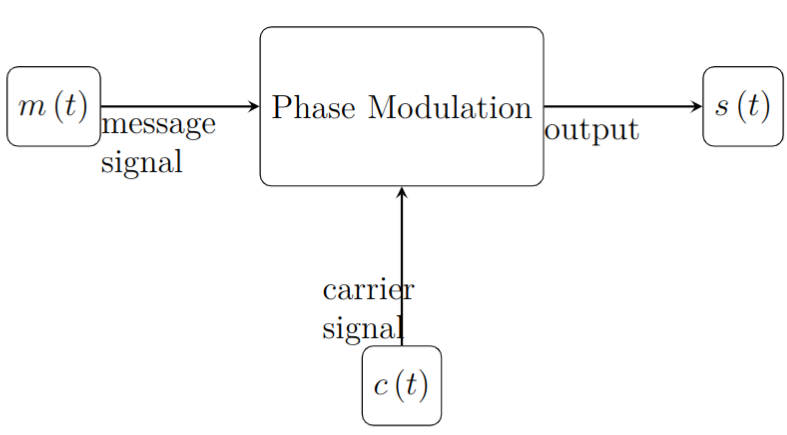
\includegraphics[width=\columnwidth]{2021/EC/49/figs/fig2.png}
    \caption{Block diagram of phase modulation}
    \label{fig:fig1_gate_2021_ec_49}  
\end{figure}
From Table \ref{tab:tab1_gate_2021_ec_49}, \ref{tab:tab2_gate_2021_ec_49} and using eq (\ref{eq:test2_21_ec49}) instantaneous frequency is given as,
\begin{align}
    f_i\brak{t} &= f_c + \frac{1}{2\pi}\, \frac{d}{dt}\theta_i\brak{t}\\
    &= f_c + \frac{1}{2\pi}\, \frac{d}{dt}\sbrak{k_p m\brak{t}}\\
    &= f_c + \frac{1}{2\pi}\, \frac{d}{dt}\brak{4\sqrt{2}\sin \brak{2 \pi 10^3 t}}\\
    &= f_c + \frac{2}{2\pi}\, 4\sqrt{2}\, \brak{2\pi 10^3}\, \brak{\cos \brak{2 \pi 10^3 t}}\\
    &= 1000 + 8\sqrt{2} \text{ x } 10^3 \cos \brak{2\pi 10^3 t}
\end{align}
Thus,
\begin{align}
    \implies f_{i_{max}} &= 1011313.7 \, Hz
\end{align}

\begin{figure}[ht]
    \centering
        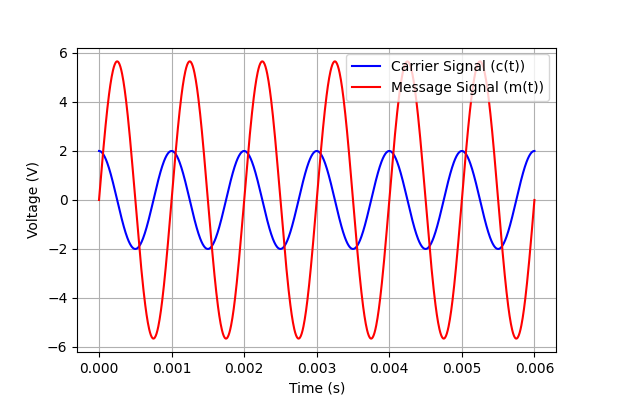
\includegraphics[width=\columnwidth]{2021/EC/49/figs/Figure_1.png}
    \caption{plot of $m\brak{t}$ and $c\brak{t}$}
\end{figure}

%\end{document}
